\chapter{Mengenal Kecerdasan Buatan dan Scikit-Learn}
Buku umum yang digunakan adalah \cite{russell2016artificial} dan  
untuk sebelum UTS menggunakan buku \textit{Python Artificial Intelligence Projects for Beginners}\cite{eckroth2018python}.
Dengan praktek menggunakan python 3 dan editor anaconda dan library python scikit-learn.
Tujuan pembelajaran pada pertemuan pertama antara lain:
\begin{enumerate}
\item
Mengerti definisi kecerdasan buatan, sejarah kecerdasan buatan, perkembangan dan penggunaan di perusahaan
\item
Memahami cara instalasi dan pemakaian sci-kit learn
\item
Memahami cara penggunaan variabel explorer di spyder
\end{enumerate}
Tugas dengan cara dikumpulkan dengan pull request ke github dengan menggunakan latex pada repo yang dibuat oleh asisten riset.

\section{Teori}
Praktek teori penunjang yang dikerjakan :
\begin{enumerate}
\item
Buat Resume Definisi, Sejarah dan perkembangan Kecerdasan Buatan, dengan bahasa yang mudah dipahami dan dimengerti. Buatan sendiri bebas plagiat[hari ke 1](10)
\item
Buat Resume mengenai definisi supervised learning, klasifikasi, regresi dan unsupervised learning. Data set, training set dan testing set.[hari ke 1](10)
\end{enumerate}

\section{Instalasi}
Membuka https://scikit-learn.org/stable/tutorial/basic/tutorial.html. Dengan menggunakan bahasa yang mudah dimengerti dan bebas plagiat. 
Dan wajib skrinsut dari komputer sendiri.
\begin{enumerate}
\item
Instalasi library scikit dari anaconda, mencoba kompilasi dan uji coba ambil contoh kode dan lihat variabel explorer[hari ke 1](10)
\item
Mencoba Loading an example dataset, menjelaskan maksud dari tulisan tersebut dan mengartikan per baris[hari ke 1](10)
\item
Mencoba Learning and predicting, menjelaskan maksud dari tulisan tersebut dan mengartikan per baris[hari ke 2](10)
\item
mencoba Model persistence, menjelaskan maksud dari tulisan tersebut dan mengartikan per baris[hari ke 2](10)
\item 
Mencoba Conventions, menjelaskan maksud dari tulisan tersebut dan mengartikan per baris[hari ke 2](10)
\end{enumerate}


\section{Penanganan Error}
Dari percobaan yang dilakukan di atas, apabila mendapatkan error maka:

\begin{enumerate}
	\item
	skrinsut error[hari ke 2](10)
	\item
Tuliskan kode eror dan jenis errornya [hari ke 2](10)
	\item
Solusi pemecahan masalah error tersebut[hari ke 2](10)

\end{enumerate}

<<<<<<< HEAD
\section{Andri Fajar S/1164065}
\subsection{sejarah dan perkembangan kecerdasan buatan}
\begin{enumerate}
\item didefinisikan  kecerdasan yang ditunjukkan oleh suatu entitas buatan. Umumnya dianggap komputer. Kecerdasan Buatan (Artificial Intelligence atau AI) didefinisikan sebagai kecerdasan yang ditunjukan oleh suatu entitas buatan. Sistem seperti ini umumnnya dianggao kemputer. Kecerdasan dimasukkan ke dalam mesin (komputer) agar dapat melakukan pekerjaan seperti yang dapat dilakukan manusia. Kecerdasan Buatan (Artificial Intelligence atau AI) didefinikasikan sebagai kecerdasan yang ditinjukkan oleh suatu entitas buatan. Sistem seperti ini umumnya di anggap komputer. Kecerdasan diciptakan dan dimasukkan melakukan pekerjaan seperti yang dapat dilakukan manusia. 
\item Sejarah dan perkembangan kecerdasan buatan terjadi pada musim panas tahun 1956 tercatat adanya seminar mengenai AI di Darmouth College. Seminar pada waktu itu dihadiri oleh sejumlah pakar komputer dan membahas potensi komputer dalam meniru 
kepandaian manusia. Akan tetapi perkembangan yang sering terjadi semenjak diciptakannya LISP, yaitu bahasa kecerdasan buatan yang dibuat tahun 1960 oleh John McCarthy. Istilah pada kecerdasan buatan atau Artificial Intelligence diambil dari Marvin Minsky dari MIT. Dia menulis karya ilmiah berjudul Step towards Artificial Intelligence,The Institute of radio Engineers Proceedings 49, January 1961\cite{ai2011kecerdasani}.
\item Supervised learning merupakan sebuah pendekatan dimana sudah terdapat data yang dilatih, dan terdapat variable yang ditargetkan sehingga tujuan dari pendekatan ini adalah mengkelompokan suatu data ke data yang sudah ada. Sedangkan unsupervised 
learning tidak memiliki data latih, sehingga dari data yang ada, kita mengelompokan data tersebut menjadi 2 bagian atau 3 bagian dan seterusnya.
\item Klasifikasi adalah salah satu topik utama dalam data mining atau machine learning. Klasifikasi yaitu suatu pengelompokan data dimana data yang digunakan tersebut mempunyai kelas label atau target.
\item Regresi adalah Supervised learning tidak hanya mempelajari classifier, tetapi juga mempelajari fungsi yang dapat memprediksi suatu nilai numerik. Contoh, ketika diberi foto seseorang, kita ingin memprediksi umur, tinggi, dan berat orang yang ada pada foto tersebut.
\item Data set adalah cabang aplikasi dari Artificial Intelligence/Kecerdasan Buatan yang fokus pada pengembangan sebuah sistem yang mampu belajar sendiri tanpa harus berulang kali di program oleh manusia.
\item Training set yaitu jika pasangan objek, dan kelas yang menunjuk pada objek tersebut adalah suatu contoh yang telah diberi label akan menghasilkan suatu algoritma pembelajaran.
\subitem Testing set digunakan untuk mengukur sejauh mana classifier berhasil melakukan klasifikasi dengan benar\cite{darujati2012pemanfaatan}.



\end{enumerate}

\subsection{INSTALASI}
Instalasi library scikit dari anaconda, mencoba kompilasi contoh kode dan lihat variable explorer.
\begin {enumerate}
\par
\item Install Aplikasi anaconda
\item buka cmd, lalu install library scikit. ketikan perintah conda install scikit-learn 
\par
\begin{figure}[ht]
\centering
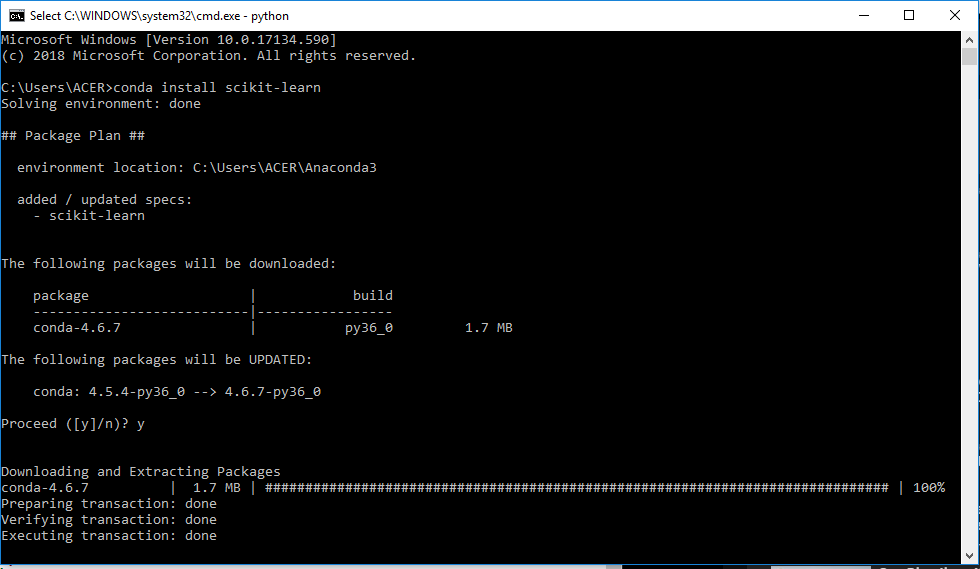
\includegraphics[scale=0.5]{figures/111.png}
\caption{Install library scikit}
\label{contoh1}
\end{figure}
\par

\item cek version anaconda dan python
\par
\begin{figure}[ht]
\centering
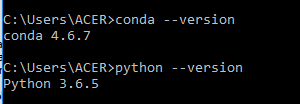
\includegraphics[scale=0.7]{figures/222.png}
\caption{version anaconda dan python}
\label{contoh2}
\end{figure}
\par

\item update library scikit dengan perintah pip install -U scikit-learn
\par
\begin{figure}[ht]
\centering
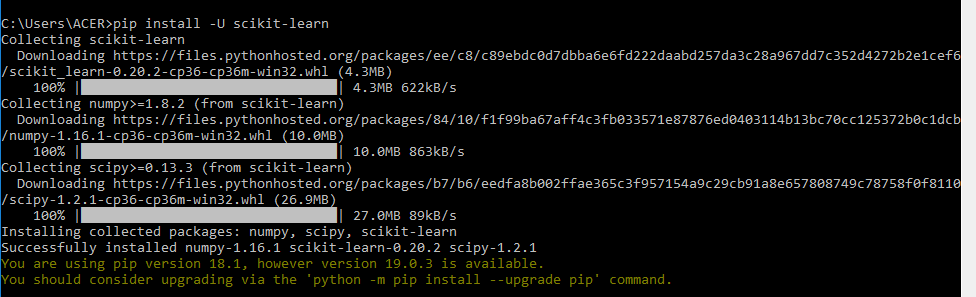
\includegraphics[scale=0.5]{figures/333.png}
\caption{update library scikit}
\label{contoh3}
\end{figure}
\par

\item test compile
\par
\begin{figure}[ht]
\centering
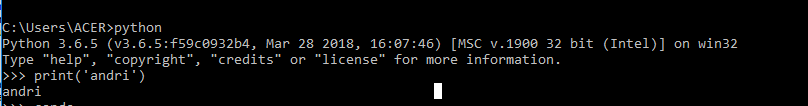
\includegraphics[scale=0.5]{figures/444.png}
\caption{test compile}
\label{contoh4}
\end{figure}
\end {enumerate}
\par

Mencoba Loading an example dataset
\begin {enumerate}
\par
\item Dari skalearn menginport dataset kemudian dataset nge load dari iris dan digits
\par
\begin{figure}[ht]
\centering
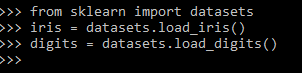
\includegraphics[scale=0.5]{figures/555.png}
\caption{import dataset}
\label{contoh5}
\end{figure}
\par
\item mencoba menampilkan data digits
\par
\begin{figure}[ht]
\centering
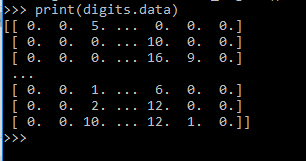
\includegraphics[scale=0.5]{figures/666.png}
\caption{data digits}
\label{contoh6}
\end{figure}
\end {enumerate}
=======
<<<<<<< HEAD
\section{Yusniar Nur Syarif Sidiq/1164089}
\subsection{Teori}
\begin{enumerate}
\item
Definisi, Sejarah, Dan Perkembangan Sejarah AI
\subitem
Kecerdasan buatan merupakan sebuah bidang dalam ilmu computer yang begitu penting di zaman ini dan masa yang akan datang guna mewujudkan sebuah sistem computer yang begitu cerdas. Kecerdasan buatan sudah berkembang begitu pesat dalam 20 tahun terakhir seiring dengan adanya kebutuhan perangkat yang cerdas pada bidang industry dan rumah tangga.
\subitem
Artificial Intelligence atau biasa di singkat dengan AI berasal dari bahasa latin yang dimana intelligence berarti saya paham. AI dimulai dari kemunculan sebuah komputer pada tahun 1940-an, akan tetapi perkembangannya dapat dilacak pada zaman Mesir Kuno. Dalam masa ini dimana perhatian difokuskan dengan kemampuan komputer dalam mengerjakan sesuatu yang dapat dilakukan oleh manusia sehingga kompute tersebut dapat meniru kemampuan dan prilaku manusia secara cerdas.
\subitem
Pada tahun 1955, Newell dan juga Simon telah mengembangkan The Logic Theorist, yaitu program AI pertama. Dimana program tersebut mempresentasikan sebuah masalah sebagai model pohon, lalu diselesaikan dengaan cara memilih cabang yang akan mewujudkan kesimpulan terbenar dan tepat. Program AI tersebut berdampak sangat besar dan dapat mendaji batu loncatan yang cukup penting dalam mengembangkan bidang AI. Sekitar tahun 1956 dimana orang yang dianggap sebagai bapak AI yaitu John McCarthy telah menyelenggarakan konferensi guna menarik para ahli dibidang komputer untuk bertemu, dengan acara yang diberi nama The Dartmouth Summer Research Project On Artificial Intelligence. Dalam konferensi tersebut telah mempertemukan pendiri dan pengembang AI. Pada konferensi tersebut bapak AI John McCarthy mengusulkan definisi AI yaitu merupakan cabang dari sebuah ilmu komputer yang dapat berfokus terhadap pengembangan computer sehingga dapat memiliki kemampuan dan juga prilaku seperti manusia.\cite{baraja2008kecerdasan}.

\item
Definisi Supervised Learning, Unsupervised Learning, Klasifikasi, Dan Regresi
\subitem
Supervised Learning merupakan sebuah pendekatan yang dimana terdapat data dan variable yang telah ditargetkan sehingga pendekatan tersebut bertujuan untuk mengelompokkan sebuah data ke data yang sudah ada, beda dengan Unsupervised learning yang tidak mempunyai data, sehingga data yang ada harus di kelompokkan menjadi beberapa bagian.
\subitem
Klasifikasi merupakan sebuah kegiatan penggolongan atau pengelompokkan. Menurut kamus besar bahasa Indonesia yang dimana klasifikasi merupakan penyusunan sistem di dalam kelompok atau golongan berdasarkan kaidah atau standar yang telah ditetapkan. Regresi merupakan sebuah metode analisis statistic yang akan digunakan untuk melihat pengaruh variable.

\item
Devinisi Dataset, Training Set, Dan Testing Set
\subitem
Dataset merupakan sebuah objek yang akan mempresentasikan sebuah data dan relasinya di memory. Struktur pada dataset ini mirip dengan data yang ada di dalam database. Training set merupakan bagian dari dataset yang berperan dalam membuat prediksi atau algoritma sesuai tujuan masing – masing. Testing set merupakan bagian dari dataset yang akan di tes guna melihat keakuratatan atau ketepatan datanya.

\subsection{Instalasi}

\begin{itemize}
\item
Memberikan perintah conda install scikit-learn di cmd, lihat gambar 1.1
\item
Melihat versinya dengan memberikan perintah conda --version dan python --version, lihat gambar 1.2
\item
Install pip, lihat pada gambar 1.3
\item
Hasil Kompile, lihat gambar 1.4
\end{itemize}

\begin{figure}[ht]
\centerline{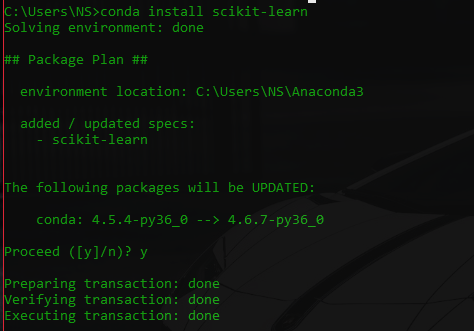
\includegraphics[width=1\textwidth]{figures/32.PNG}}
\caption{conda install scikit-learn.}
\end{figure}

\begin{figure}[ht]
\centerline{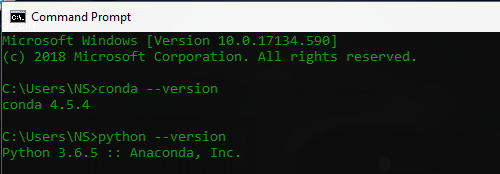
\includegraphics[width=1\textwidth]{figures/31.PNG}}
\caption{Melihat Version.}
\end{figure}

\begin{figure}[ht]
\centerline{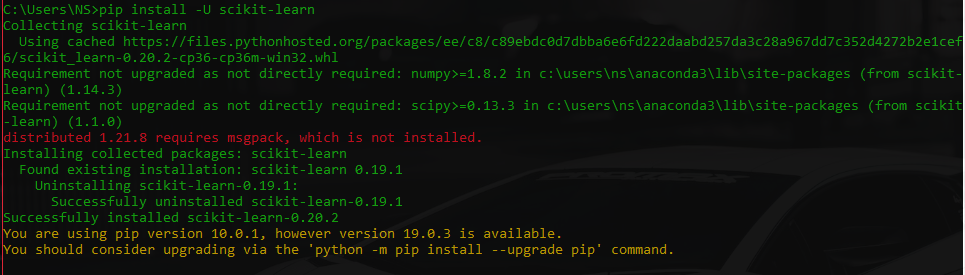
\includegraphics[width=1\textwidth]{figures/33.PNG}}
\caption{Install pip.}
\end{figure}

\begin{figure}[ht]
\centerline{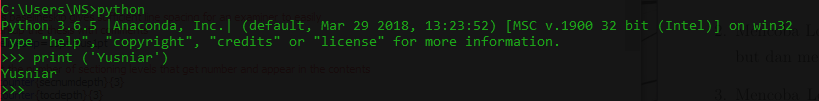
\includegraphics[width=1\textwidth]{figures/35.PNG}}
\caption{Hasil Kompile.}
\end{figure}

\subitem
Dataset adalah objek seperti kamus yang menyimpan semua data dan berupa metadata tentang data. Data tersebut disimpan di .data anggota yang merupakan array. Misalnya dalam kasus dataset digit, memberikan akses ke fitur yang dapat digunakan untuk mengklarifikasikan sempel digit, lihat gambar 1.5.

\begin{figure}[ht]
\centerline{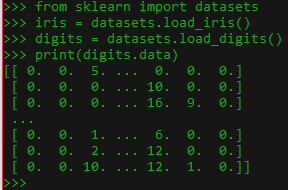
\includegraphics[width=1\textwidth]{figures/36.PNG}}
\caption{Dataset.}
\end{figure}

\subsection{Learning And Predicting}
\begin{verbatim}

from sklearn import datasets
iris = datasets.load_iris()
digits = datasets.load_digits()
from sklearn import svm
clf = svm.SVC(gamma=0.0001, C=100.)
clf.fit(digits.data[:-1], digits.target[:-1])
clf.predict(digits.data[-1:])

\end{verbatim}
\subitem
Pada baris pertama akan melakukan import datasets dari folder sklearn.
Pada baris kedua akan mengambil datasets iris dari folder iris
Pada baris ketiga yaitu akan mengambil datasets digit dari folder digit
Pada baris keempat akan melakukan import svm dari folder sklearn
Pada baris Kelimla akan melakukan deklarasi gamma
Pada baris kenam akan membaca data digits dan target digits
Pada baris ketujuh akan melakukan prediksi data

\subsection{ Model Persistence}

\begin{verbatim}

from sklearn import svm
from sklearn import datasets
 clf = svm.SVC(gamma='scale')
 iris = datasets.load_iris()
 X, y = iris.data, iris.target
 clf.fit(X, y)  
SVC(C=1.0, cache_size=200, class_weight=None, coef0=0.0,
  decision_function_shape='ovr', degree=3, gamma='scale', kernel='rbf',
  max_iter=-1, probability=False, random_state=None, shrinking=True,
  tol=0.001, verbose=False)

import pickle
 s = pickle.dumps(clf)
 clf2 = pickle.loads(s)
 clf2.predict(X[0:1])
array([0])
 y[0]
0

\end{verbatim}
\subitem
Pada baris pertama akan melakukan import svm dari folder sklearn
Pada baris kedua akan melakukan import datasets dari folder sklearn
Pada baris ketiga akan mendeklarasikan gamma dengan scale
Pada baris keempat akan mengambil datasets iris dari folder iris
Pada bari kelima akan mendeklarasikan data iris dan target iris dengan X dan y
Pada baris ke delapan akan melakukan import pickle
Pada baris kesembilan akan memanggil deklarasi scale dengan s
Pada baris kesepuluh akan mengambil data pickle
Pada baris berikutnya akan melakukan prediksi dan memunculkan hasilnya

\subsection{Conventions}
\begin{verbatim}
1.
import numpy as np
from sklearn import random_projection

 rng = np.random.RandomState(0)
 X = rng.rand(10, 2000)
 X = np.array(X, dtype='float32')
 X.dtype
dtype('float32')

 transformer = random_projection.GaussianRandomProjection()
 X_new = transformer.fit_transform(X)
 X_new.dtype
dtype('float64')

\end{verbatim}
\subitem
Pada baris pertama akan melakukan import numpy.
Pada baris berikutnya akan melakukan import akan tetapi dengan data yang random pada folder sklearn.
Pada baris berikutnya akan menentukan nilan array dan radian pada X.
Pada baris berikutnya menentukan type data X.
Pada baris berikutnya dijelaskan bahwa typenya yaitu float 32.
Pada baris berikunya akan menentukan random project dengan menggunakan transformer.
Baris berikutnya membuat nilai X baru dan mengirimnya dengan menggunakan transformer.fit\_transform.
Pada baris berikutnya membuat type baru pada X.
Pada baris berikutnya hasil dari type tersebut adalah float64.

\begin{verbatim}

2.
 from sklearn import datasets
 from sklearn.svm import SVC
 iris = datasets.load_iris()
 clf = SVC(gamma='scale')
 clf.fit(iris.data, iris.target)  
SVC(C=1.0, cache_size=200, class_weight=None, coef0=0.0,
  decision_function_shape='ovr', degree=3, gamma='scale', kernel='rbf',
  max_iter=-1, probability=False, random_state=None, shrinking=True,
  tol=0.001, verbose=False)

 list(clf.predict(iris.data[:3]))
[0, 0, 0]

 clf.fit(iris.data, iris.target_names[iris.target])  
SVC(C=1.0, cache_size=200, class_weight=None, coef0=0.0,
  decision_function_shape='ovr', degree=3, gamma='scale', kernel='rbf',
  max_iter=-1, probability=False, random_state=None, shrinking=True,
  tol=0.001, verbose=False)

 list(clf.predict(iris.data[:3]))  
['setosa', 'setosa', 'setosa']

\end{verbatim}
\subitem
Pada baris pertama melakukan importdatasets dari folder sklearn.
Pada baris berikutnya akan melakukan import SVC dari folder sklearn.
Pada baris berikutnya akan mengambil datasets iriis dari folder iris.
Pada baris berikutnya akan melakukan deklarasi pada gamma
Pada baris berikutnya membaca data iris dan target iris.
Pada baris berikutnya akan melakukan prediksi dan hasilnya adalah 0,0,0.
Pada baris berikutnya akan memberikan nama pada setiap data iris.
Pada baris berikutnya akan melakukan prediksi dan akan memunculkan hasilnya.

\subsection{Refitting And Updating Parameters}

\begin{verbatim}

import numpy as np
from sklearn.svm import SVC

rng = np.random.RandomState(0)
 X = rng.rand(100, 10)
 y = rng.binomial(1, 0.5, 100)
 X_test = rng.rand(5, 10)

 clf = SVC()
 clf.set_params(kernel='linear').fit(X, y)  
SVC(C=1.0, cache_size=200, class_weight=None, coef0=0.0,
  decision_function_shape='ovr', degree=3, gamma='auto_deprecated',
  kernel='linear', max_iter=-1, probability=False, random_state=None,
  shrinking=True, tol=0.001, verbose=False) clf.predict(X_test)
array([1, 0, 1, 1, 0])

 clf.set_params(kernel='rbf', gamma='scale').fit(X, y)  
SVC(C=1.0, cache_size=200, class_weight=None, coef0=0.0,
  decision_function_shape='ovr', degree=3, gamma='scale', kernel='rbf',
  max_iter=-1, probability=False, random_state=None, shrinking=True,
  tol=0.001, verbose=False)
 clf.predict(X_test)
array([1, 0, 1, 1, 0])

\end{verbatim}
\subitem
Pada baris pertama akan melakukan import pada numpy.
Pada baris selanjutnya akan melakukan import SVC dari folder sklearn.
Pada baris berikutnya akan menentukan nilai dari RandomState.
Pada baris berikutnya akan menentukan metode yang digunakan yaitu linier dan akan membaca data SVC.
Hasilnya berupa da array.

\subsection{Multiclass VS Multilabel Fitting}

\begin{verbatim}
1.
 from sklearn.svm import SVC
 from sklearn.multiclass import OneVsRestClassifier
 from sklearn.preprocessing import LabelBinarizer

 X = [[1, 2], [2, 4], [4, 5], [3, 2], [3, 1]]
 y = [0, 0, 1, 1, 2]
classif = OneVsRestClassifier(estimator=SVC(gamma='scale', random_state=0))
classif.fit(X, y).predict(X)
array([0, 0, 1, 1, 2])
\end{verbatim}
\subitem
Pada baris pertama akan melakukan import SVC pada folder sklearn.
Pada baris berikutnya akan melakukan import class.
Class yang digunakan adalah OneVsRestClassifier sehingga akan menciptakan outputan array.
\begin{verbatim}
2.
 y = LabelBinarizer().fit_transform(y)
classif.fit(X, y).predict(X)
array([[1, 0, 0],
       [1, 0, 0],
       [0, 1, 0],
       [0, 0, 0],
       [0, 0, 0]])
\end{verbatim}
\subitem
Codingan tersebut akan membaca output pada label dan akan mengeluarkan data array.
\begin{verbatim}
3.
from sklearn.preprocessing import MultiLabelBinarizer
y = [[0, 1], [0, 2], [1, 3], [0, 2, 3], [2, 4]]
y = MultiLabelBinarizer().fit_transform(y)
classif.fit(X, y).predict(X)
array([[1, 1, 0, 0, 0],
       [1, 0, 1, 0, 0],
       [0, 1, 0, 1, 0],
       [1, 0, 1, 0, 0],
       [1, 0, 1, 0, 0]])
\end{verbatim}
\subitem
Pada baris pertama akan melakukan import Multilabelbinarizer yang berisikan data-data lalu di transform sehingga memunculkan data array.

\subsection{Penjelasan Eror}
\subitem
Dimana Erorr Tersebut dapat di lihat pada gambar Figure Joblib Erorr

\begin{figure}[ht]
\centerline{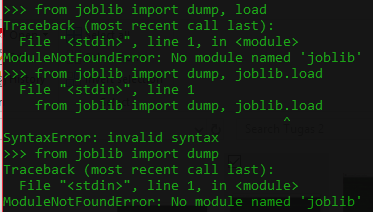
\includegraphics[width=1\textwidth]{figures/Joblib Erorr Y.PNG}}
\caption{Joblib Erorr.}
\end{figure}

\subitem
Codingan yang eror tersebut adalah
\begin{verbatim}
from joblib import dump, load
\end{verbatim}
\subitem
Hal ini dikarenakan belum terinstallnya file joblib di dalam pc anda. Untuk menginstallnya cukup berikan perintah
\begin{verbatim}
pip install joblib
\end{verbatim}

\subitem
maka hasilnya akan nampak sepeti pada gambar hasil joblib

\begin{figure}[ht]
\centerline{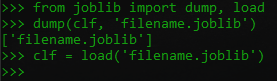
\includegraphics[width=1\textwidth]{figures/Hasil Joblib Y.PNG}}
\caption{Hasil Joblib.}
\end{figure}
\end{enumerate}






=======
\section{Imron Sumadireja / 1164076}
\subsection{Teori}
\begin{enumerate}
\item
Pengertian
\subitem
Kecerdasan Buatan Artificial Intelligence merupakan salah satu bagian dari ilmu komputer yang mempelajari cara membuat mesin komputer dapat melakukan pekerjaan sebaik bahkan lebih baik dari yang dilakukan oleh manusia. Agar mesin dapat bekerja layaknya manusia maka perlu diberi bekal pengetahuan, sehingga mempunyai kemampuan untuk menalar. Menurut para ahli kecerdasan buatan seperti berikut:
\begin{itemize}
\item
H. A. Simon:
Kecerdasan buatan Artificial Intelligence merupakan kawasan penelitian, aplikasi dan instruksi yang terkait dengan pemrograman komputer untuk melakukan sesuatu hal yang dalam pandangan manusia adalah cerdas.
\item
Rich and Knight:
Kecerdasan buatan Artificial Intelligence merupakan sebuah studi tentang bagaimana membuat komputer melakukan hal-hal yang pada saat ini dapat dilakukan lebih baik oleh manusia.
\end{itemize}

\item
Sejarah dan Perkembangan
\subitem
Kata intelligence berasal dari bahasa latin intelligo yang memiliki arti saya paham. Arti dasar dari intelligence merupakan kemampuan untuk memahami dan melakukan aksi. Area Kecerdasan Buatan Artificial Intelligence, bermula pada saat kemunculan komputer sekitar tahun 1940-an, walaupun sejarah perkembangannya dapat dilacak sejak zaman Mesir kuno. Pada masa saat ini, perhatian difokuskan pada kemampuan komputer mengerjakan sesuatu yang dapat dilakukan oleh manusia. Dalam hal ini, komputer tersebut dapat meniru kemampuan kecerdasan dan perilaku manusia dengan akurasi yang cukup baik \cite{warwick2013artificial}.
\subitem
Pada akhir tahun 1955, Newell dan Simon mengembangkan The Logic Theorist, program AI pertama, program ini merepresentasikan masalah sebagai model pohon, lalu penyelesaiannya dengan memilih cabang yang akan menghasilkan kesimpulan yang paling benar. Pada tahun 1956 John McCarthy dari Massacuhetts Institute of Technology dianggap sebagai bapak AI, menyelenggarakan konferensi untuk menarik para ahli komputer bertemu, dengan nama kegiatan The Dartmouth Summer Research Project on Artificial Intelligence. Konferensi Dartmouth itu mempertemukkan para pendiri AI, dan bertugas untuk meletakkan dasar bagi masa depan pengembangan dan penelitian AI. John McCarthy saat itu mengusulkan definisi AI adalah AI merupakan cabang dari ilmu komputer yang berfokus pada pengembangan komputer untuk dapat memiliki kemampuan dan berprilaku seperti manusia\cite{bassil2012expert}.

\item
Supervised Learning dan Unsupervised Learning
\subitem
Supervised Learning merupakan suatu pendekatan dimana sudah terdapat data yang dilatih, dan terdapat variable yang ditargetkan sehingga tujuan dari pendekatan ini adalah mengelompokan suatu data ke data yang sudah ada. Sebagai contoh, ketika Anda memiliki sejumlah buku yang sudah dibeli dengan beberapa kategori. Misalnya, kategori buku akademik, dan buku novel. Selanjutnya Anda membeli sejumlah buku baru, maka Anda harus mengindentifikasi buku tersebut, dan memasukannya dalam kategori yang sudah ada.
\subitem
Unsupervised Learning merupakan suatu pendekatan namun tidak memiliki data yang dilatih, sehingga dari data yang ada, kita dapat mengelompokan data tersebut menjadi 2 bagian atau 3 bagian dan seterusnya. Sebagai contoh, Anda belum pernah membeli sejumlah buku, suatu hari Anda membeli sejumlah buku dan ingin membaginya kedalam beberapa kategori agar mudah dicari. Anda akan mengidentifikasi buku mana yang mirip. Dalam hal ini, kita memilih buku berdasarkan isinya.


\item
Klasifikasi dan Regresi
\subitem
Klasifikasi merupakan penempatan objek-objek ke salah satu dari beberapa kategori yang telah ditentukan sebelumnya. Klasifikasi banyak digunakan untuk memprediksi kelas pada suatu label atau atribut tertentu, yaitu dengan mengklasifikasi data membangun model berdasarkan training set dan nilai-nilai dalm mengklasifikasikan data yang baru.
Regresi dibedakan menjadi 2, diantaranya regresi linear dan regresi nonlinear.
\begin{itemize}
\item
Regresi Linear
Regresi Linear merupakan bentuk hubungan di mana variabel bebas x maupun variabel tergantung y sebagai faktor yang berpangkat satu.
\item
Regresi Nonlinear
Regresi Nonlinear merupakan bentuk hubungan atau fungsi di mana variabel x dan variabel tidak bebas y dapat berfungsi sebagai faktor atau variabel dengan pangkat tertentu.
\end{itemize}

\item
Data set, Training set, dan Testing set
\subitem
Untuk melakukan data set, training set, dan testing set diperlukan beberapa langkah, diantaranya:
\begin{itemize}
\item
Membuat model atau mesin untuk memeriksa data,
\item
Membuat model atau mesin belajar dari kesalahannya,
\item
Membuat kesimpulan tentang sebarapa baik kinerja model atau mesin tersebut.
\end{itemize}

\begin{enumerate}
\item
Data set
\subitem
Data set ini mencakup sekumpulan contoh input yang modelnya akan cocok atau dilatih dengan menyesuaikan parameter.
\item
Training set
\subitem
Training set diperlukan oleh model atau mesin agar dapat dilatih. Dengan menghitung kerugian tingkat kesalahan yang dilakukan model atau mesin menghasilkan pada set validasi pada titik tertentu, agar kita tahu seberapa akuratnya. Selanjutnya, model akan menyesuaikan parameternya berdasarkan hasil evaluasi yang sering pada training set ini.
\item
Testing set
\subitem
Testing set sangat penting untuk menguji generelasi model atau mesin. Dengan testing set ini, kita bisa mendapatkan akurasi kinerja model atau mesin.
\end{enumerate}

\end{enumerate}

\subsection{Instalasi}
\subsubsection{Proses Instalasi Anaconda dan Library Scikit}
\begin{enumerate}
\item Pertama kita unduh terlebih dahulu aplikasi anaconda, seperti gambar berikut
\begin{figure}[ht]
\centering
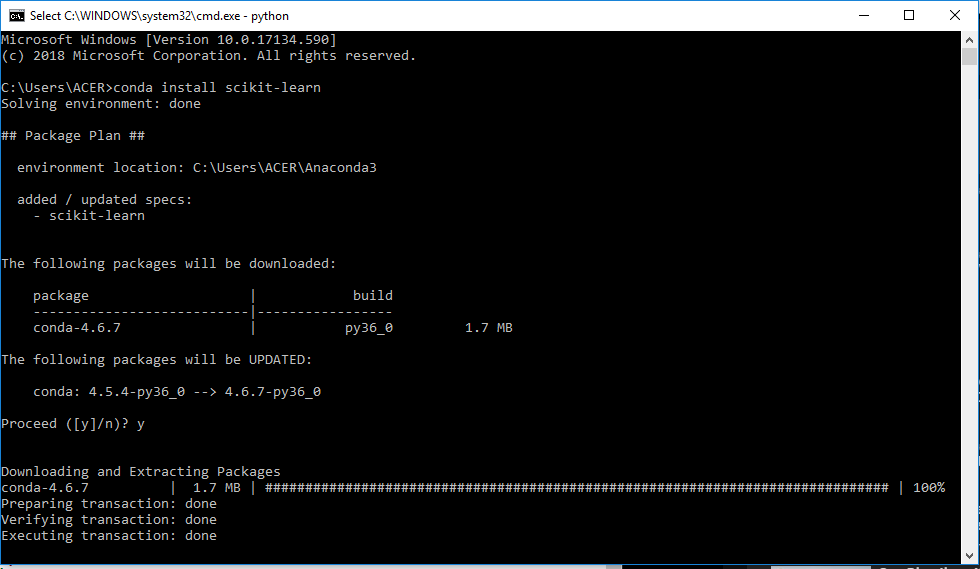
\includegraphics[scale=0.3]{figures/1.png}
\caption{Download Aplikasi Anaconda}
\end{figure}

\item Setelah di unduh, selanjutnya buka aplikasi tersebut. Lalu klik next untuk melanjutkan.
\begin{figure}[ht]
\centering
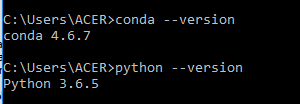
\includegraphics[scale=0.7]{figures/2.png}
\caption{Proses Instalasi Aplikasi}
\end{figure}

\item Lalu klik I Agree untuk melanjutkan.
\begin{figure}[ht]
\centering
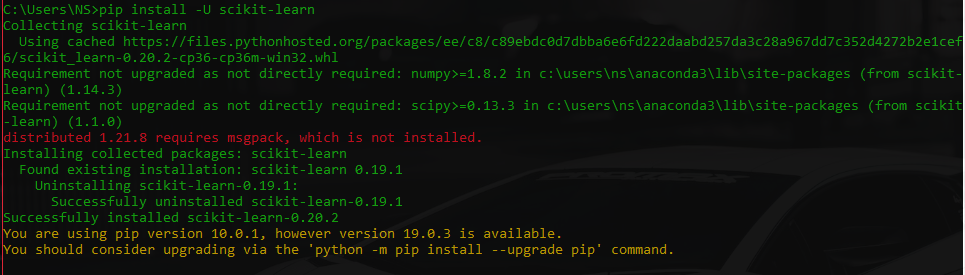
\includegraphics[scale=0.7]{figures/3.png}
\caption{Proses Instalasi Aplikasi}
\end{figure}

\item Selanjutnya pilih Just me agar aplikasi tersebut hanya dapat digunakan oleh user yang login pada laptop tersebut.
\begin{figure}[ht]
\centering
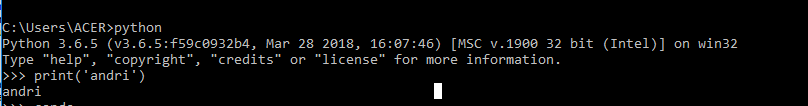
\includegraphics[scale=0.7]{figures/4.png}
\caption{Proses Instalasi Aplikasi}
\end{figure}

\item Lalu tentukan direktori penyimpanan file tersebut
\begin{figure}[ht]
\centering
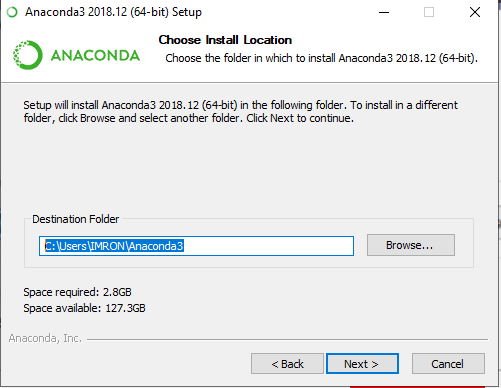
\includegraphics[scale=0.7]{figures/5.png}
\caption{Proses Instalasi Aplikasi}
\end{figure}

\item Selanjutnya akan muncul pop up box tentang advance installation options, ceklis keduanya.
\begin{figure}[ht]
\centering
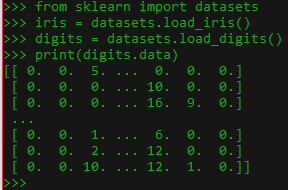
\includegraphics[scale=0.7]{figures/6.png}
\caption{Proses Instalasi Aplikasi}
\end{figure}

\item Tunggu hingga proses install selesai
\begin{figure}[ht]
\centering
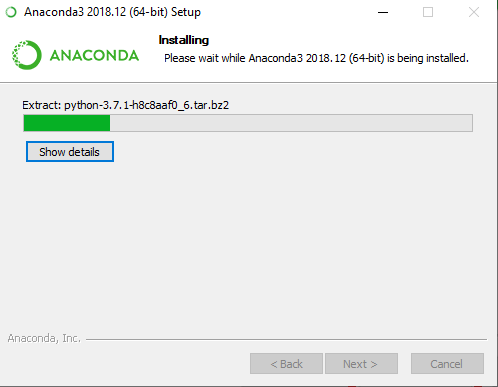
\includegraphics[scale=0.7]{figures/7.png}
\caption{Proses Instalasi Aplikasi}
\end{figure}

\item Setelah proses instalasi selesai, klik next
\begin{figure}[ht]
\centering
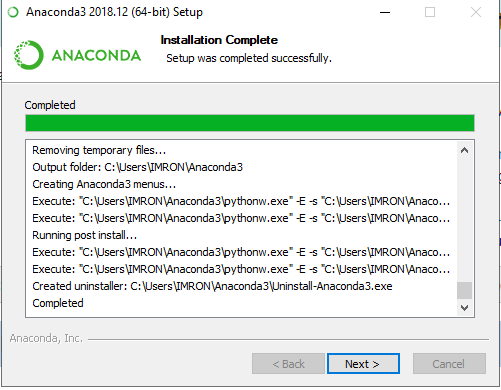
\includegraphics[scale=0.7]{figures/8.png}
\caption{Proses Instalasi Aplikasi}
\end{figure}

\item Pada bagian selanjutnya akan muncul box dengan memberikan pilihan untuk install VS Code,  jika tidak klik skip.
\begin{figure}[ht]
\centering
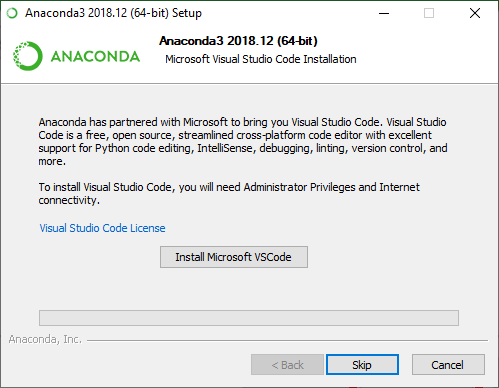
\includegraphics[scale=0.7]{figures/9.png}
\caption{Proses Instalasi Aplikasi}
\end{figure}

\item Setelah selesai, klik finish
\begin{figure}[ht]
\centering
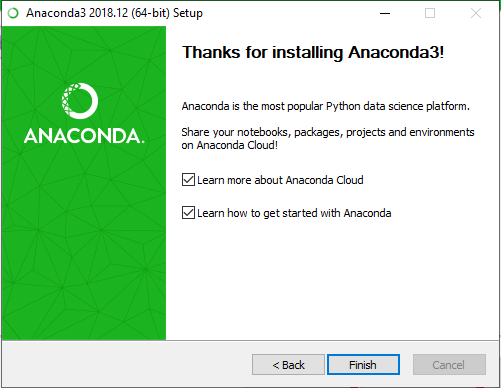
\includegraphics[scale=0.7]{figures/10.png}
\caption{Proses Instalasi Aplikasi}
\end{figure}

\item Setelah proses instalasi selesai, selanjutnya buka cmd dan ketikan seperti berikut.
\begin{figure}[ht]
\centering
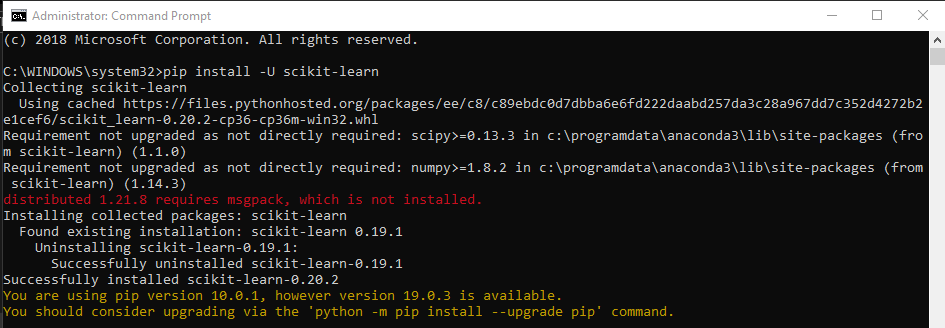
\includegraphics[scale=0.5]{figures/16.png}
\caption{Instalasi Library}
\end{figure}

\item Selanjutnya ketikan perintah berikut untuk mengunduh library scikit
\begin{figure}[ht]
\centering
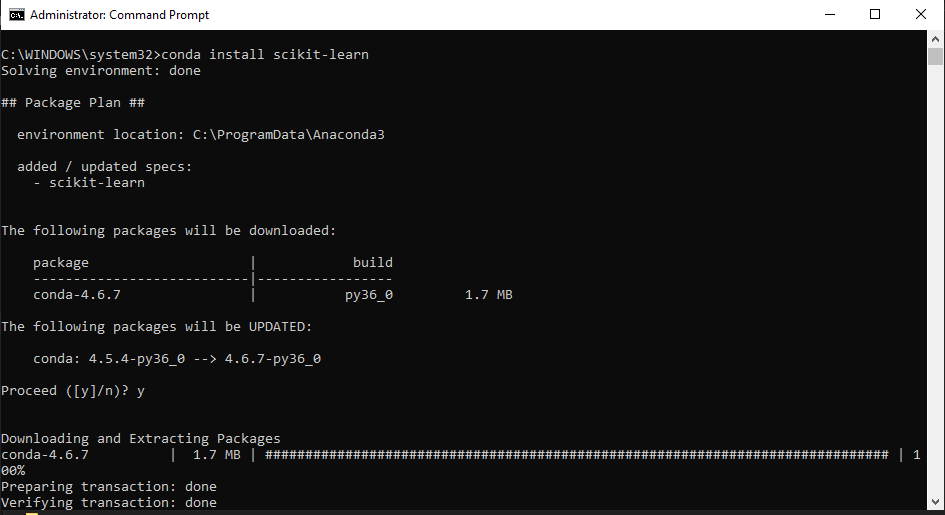
\includegraphics[scale=0.5]{figures/17.png}
\caption{Instalasi Library}
\end{figure}

\item Jika sudah berhasil selanjutnya, ketikan perintah seperti gambar berikut untuk malakukan cek versi conda dan python
\begin{figure}[ht]
\centering
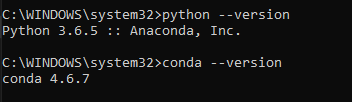
\includegraphics[scale=0.7]{figures/18.png}
\caption{Instalasi Library}
\end{figure}

\item Mencoba dan mengcompile source code, hasilnya seperti berikut
\begin{figure}[ht]
\centering
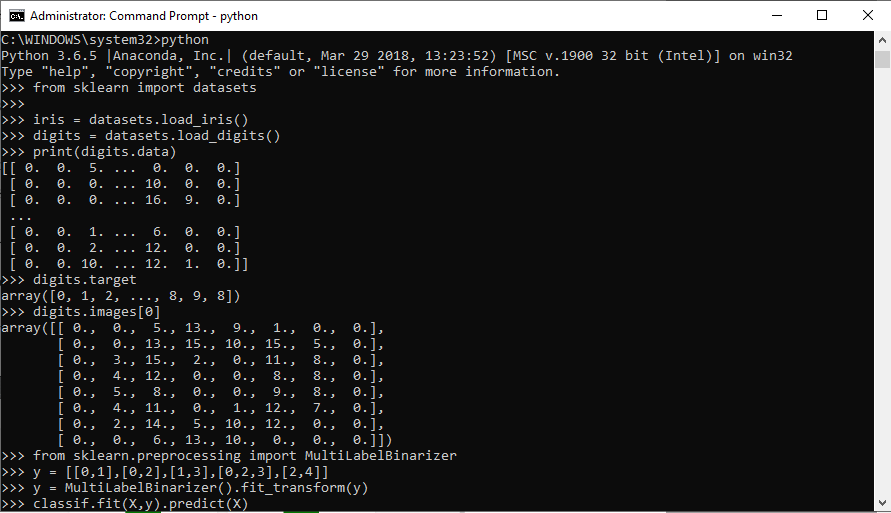
\includegraphics[scale=0.5]{figures/19.png}
\caption{Instalasi Library}
\end{figure}
\end{enumerate}

\subsection{Mencoba Loading Dataset}
\begin{enumerate}
\item Berikut source code yang menjelaskan tentang loading dataset. Pada baris pertama code tersebut berfungsi untuk import library datasets dari sklearn. Baris kedua berfungsi untuk menampilkan data secara berurutan. Baris ketiga untuk menampilkan data tersebut berupa angka dan baris keempat untuk menampilkan data tersebut.
\begin{figure}[ht]
\centering
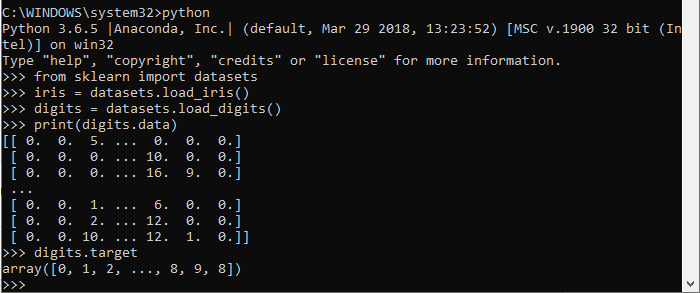
\includegraphics[scale=0.5]{figures/20.png}
\caption{Loading dataset}
\end{figure}
\end{enumerate}

\subsection{Learning and Predicting}
\begin{verbatim}
>>> from sklearn import datasets
>>> iris = datasets.load_iris()
>>> digits = datasets.load_digits()
>>> print(digits.data)
\end{verbatim}
\begin{itemize}
\item import datasets dari package sklearn
\item loading dataset iris
\item loading dataset digits
\item menampilkan data dari loading dataset digits
\begin{verbatim}
>>> from sklearn import svm
>>> clf = svm.SVC(gamma=0.001, C=100.)
>>> clf.fit(digits.data[:-1], digits.target[:-1])
\end{verbatim}
\item Baris tersebut menjelaskan bahwa dalam project ini kita menggunakan source dari sklearn dengan mengambil/import dari svm
\item classifier svc dengan atribur gamma dan c
\item classifier tersebut akan dijalanakan dengan menggunakan metode fit
\begin{verbatim}
  SVC(C=100.0, cache_size=200, class_weight=None, coef0=0.0,
  decision_function_shape='ovr', degree=3, gamma=0.001, kernel='rbf',
  max_iter=-1, probability=False, random_state=None, shrinking=True,
  tol=0.001, verbose=False)
\end{verbatim}
\item hasilnya seperti di atas
\begin{verbatim}
>>> clf.predict(digits.data[-1:])
\end{verbatim}
\item classifier predict loading data digits
\begin{verbatim}
 array([8])
\end{verbatim}
\item hasilnya seperti di atas
\end{itemize}

\subsection{Model Persistence}
\begin{verbatim}
>>> from sklearn import svm
>>> from sklearn import datasets
>>> clf = svm.SVC(gamma='scale')
>>> iris = datasets.load_iris()
>>> X, y = iris.data, iris.target
>>> clf.fit(X, y)
\end{verbatim}
\begin{itemize}
\item import svm dari package sklearn
\item importt datasets dari package sklearn
\item classifier svc dengan atribut gamma
\item loading dataset iris
\item parameter x dan y dengan key iris data dan iris target
\item classifier akan dijalankan menggunakan metode fit
\begin{verbatim}
  SVC(C=1.0, cache_size=200, class_weight=None, coef0=0.0,
  decision_function_shape='ovr', degree=3, gamma='scale', kernel='rbf',
  max_iter=-1, probability=False, random_state=None, shrinking=True,
  tol=0.001, verbose=False)
\end{verbatim}
\item hasilnya seperti di atas
\begin{verbatim}
>>> import pickle
>>> s = pickle.dumps(clf)
>>> clf2 = pickle.loads(s)
>>> clf2.predict(X[0:1])
\end{verbatim}
\item import package pickle
\item pickle akan melakukan dumps pada classifier
\item classifier2 akan mengambil data pada classifier pertama
\item classifier2 akan memprediksi hasilnya dengan menggunakan syntax python
\begin{verbatim}
array([0])
\end{verbatim}
\item hasilnya seperti diatas
\begin{verbatim}
>>> y[0]
\end{verbatim}
\item parameter y dengan atribut 0
\begin{verbatim}
 0
\end{verbatim}
\item hasil seperti di atas
\end{itemize}

\subsection{Conventions}
\begin{verbatim}
>>> import numpy as np
>>> from sklearn import random_projection
>>> rng = np.random.RandomState(0)
>>> X = rng.rand(10, 2000)
>>> X = np.array(X, dtype='float32')
>>> X.dtype
\end{verbatim}
\begin{itemize}
\item iimport numpy dengan alias np
\item import random projection pada package sklearn
\item rng parameter dan akan melakukan proses random dalam menentukan hasil
\item parameter x memiliki rand dengan nilai 10, 2000
\item parameterr x dengan numpy array akan memunculkan kata float32 pada hasil terakhir
\begin{verbatim}
dtype('float32')
\end{verbatim}
\item hasilnya seperti diatas
\begin{verbatim}
>>> transformer = random_projection.GaussianRandomProjection()
>>> X_new = transformer.fit_transform(X)
>>> X_new.dtype
\end{verbatim}
\item transformer parameter yang di gunakan untuk melakukan pencarian data dengan gaussianrandomprojection
\item x new parameter dan akan dijalankan dengan menggunakan metode fit
\item x dtype akan menampilkan hasilnya
\begin{verbatim}
dtype('float64')
\end{verbatim}
\item hasilnya seperti di atas
\begin{verbatim}
>>> from sklearn import datasets
>>> from sklearn.svm import SVC
>>> iris = datasets.load_iris()
>>> clf = SVC(gamma='scale')
>>> clf.fit(iris.data, iris.target)
\end{verbatim}
\item import datasets pada package sklearn
\item import svc pada package sklearn
\item loading dataset iris
\item classifier dengan atribut gamma
\item classifier dengan metode fit pada key iris dan target.
\begin{verbatim}
SVC(C=1.0, cache_size=200, class_weight=None, coef0=0.0,
  decision_function_shape='ovr', degree=3, gamma='scale', kernel='rbf',
  max_iter=-1, probability=False, random_state=None, shrinking=True,
  tol=0.001, verbose=False)
\end{verbatim}
\item hasilnya seperti di atas
\begin{verbatim}
>>> list(clf.predict(iris.data[:3]))
\end{verbatim}
\item untuk list classifier predict pada loading dataset iris
\begin{verbatim}
[0, 0, 0]
\end{verbatim}
\item hasilnya seperti diatas
\begin{verbatim}
>>> clf.fit(iris.data, iris.target_names[iris.target])
\end{verbatim}
\item classifier dengan menggunakan metode fit dan key data dan target
\begin{verbatim}
SVC(C=1.0, cache_size=200, class_weight=None, coef0=0.0,
  decision_function_shape='ovr', degree=3, gamma='scale', kernel='rbf',
  max_iter=-1, probability=False, random_state=None, shrinking=True,
  tol=0.001, verbose=False)
\end{verbatim}
\item hasilnya seperti diatas
\begin{verbatim}
>>> list(clf.predict(iris.data[:3]))
\end{verbatim}
\item list untuk classifier pada predict loading data iris
\begin{verbatim}
['setosa', 'setosa', 'setosa']
\end{verbatim}
\item hasilnya seperti diatas
\begin{verbatim}
>>> import numpy as np
>>> from sklearn.svm import SVC
>>> rng = np.random.RandomState(0)
>>> X = rng.rand(100, 10)
>>> y = rng.binomial(1, 0.5, 100)
>>> X_test = rng.rand(5, 10)
>>> clf = SVC()
>>> clf.set_params(kernel='linear').fit(X, y)
\end{verbatim}
\item import numpy alias np
\item import svc dari package sklearn
\item rng parameter untuk mencari data pada atribut randomstate
\item X memiliki jangakaun rand 100, 10
\item y memiliki binominal 5,10
\item x memiliki rand 5,10
\item classifier dengan atribut svc
\item classifier parameter dengan atribut linear menggunakan metode fit
\begin{verbatim}
SVC(C=1.0, cache_size=200, class_weight=None, coef0=0.0,
  decision_function_shape='ovr', degree=3, gamma='auto_deprecated',
  kernel='linear', max_iter=-1, probability=False, random_state=None,
  shrinking=True, tol=0.001, verbose=False)
\end{verbatim}
\item hasilnya seperti di atas
\begin{verbatim}
>>> clf.predict(X_test)
\end{verbatim}
\item classifier untuk memprediksi nilai x
\begin{verbatim}
array([1, 0, 1, 1, 0])
\end{verbatim}
\item hasilnya seperti di atas
\begin{verbatim}
>>> clf.set_params(kernel='rbf', gamma='scale').fit(X, y)
\end{verbatim}
\item classifier parameters dengan atribut gamma menggunakan metode fit
\begin{verbatim}
SVC(C=1.0, cache_size=200, class_weight=None, coef0=0.0,
  decision_function_shape='ovr', degree=3, gamma='scale', kernel='rbf',
  max_iter=-1, probability=False, random_state=None, shrinking=True,
  tol=0.001, verbose=False)
\end{verbatim}
\item hasilnya seperti di atas
\begin{verbatim}
>>> clf.predict(X_test)
\end{verbatim}
\item classifier prediksi dari x 
\begin{verbatim}
array([1, 0, 1, 1, 0])
\end{verbatim}
\item hasilnya seperti di atas
\begin{verbatim}
>>> from sklearn.svm import SVC
>>> from sklearn.multiclass import OneVsRestClassifier
>>> from sklearn.preprocessing import LabelBinarizer
>>> X = [[1,2],[2,4],[4,5],[3,2],[3,1]]
>>> y = [0,0,1,1,2]
>>> classif = OneVsRestClassifier(estimator=SVC(gamma='scale', random_state=0))
>>> classif.fit(X, y).predict(X)
array([0, 0, 1, 1, 2])
>>> y = LabelBinarizer().fit_transform(y)
>>> classif.fit(X, y).predict(X)
\end{verbatim}
\item import svc dari package sklearn
\item import OneVsRentClassifier dari package sklearn
\item import LabelBinarizer dari package sklearn
\item atribut x
\item atribut y
\item classifier dengan atribut OneVsRestClassifier dan estimator svc
\begin{verbatim}
array([[1, 0, 0],
       [1, 0, 0],
       [0, 1, 0],
       [0, 0, 0],
       [0, 0, 0]])
\end{verbatim}
\item hasilnya seperti di atas
\begin{verbatim}
>>> from sklearn.preprocessing import MultiLabelBinarizer
>>> y = [[0,1],[0,2],[1,3],[0,2,3],[2,4]]
>>> y = MultiLabelBinarizer().fit_transform(y)
>>> classif.fit(X, y).predict(X)
\end{verbatim}
\item import MultiLabelBinarizer dari package sklearn
\item atribut y
\item atribut y akan dijankan dengan metode fit pada tampilan MultiLabelBinarizer
\item classifier dengan metode fit pada x dan y untuk memprediksi 
\begin{verbatim}
array([[1, 1, 0, 0, 0],
       [1, 0, 1, 0, 0],
       [0, 1, 0, 1, 0],
       [1, 0, 1, 0, 0],
       [1, 0, 1, 0, 0]])
\end{verbatim}
\item hasilnya seperti di atas
\end{itemize}

\subsection{Penanganan Error}
Dari percobaan yang telah dilakukan terdapat error yang di dapatkan pada bagian joblib model persistence

\begin{figure}[ht]
\centering
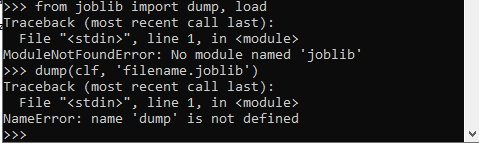
\includegraphics[scale=0.5]{figures/i20.png}
\caption{Error}
\end{figure}

\begin{itemize}
\item Error tersebut dikarenakan saya belum install package joblib sehingga error pun terjadi dengan source code sebagai berikut:
from joblib import dump, load

\begin{figure}[ht]
\centering
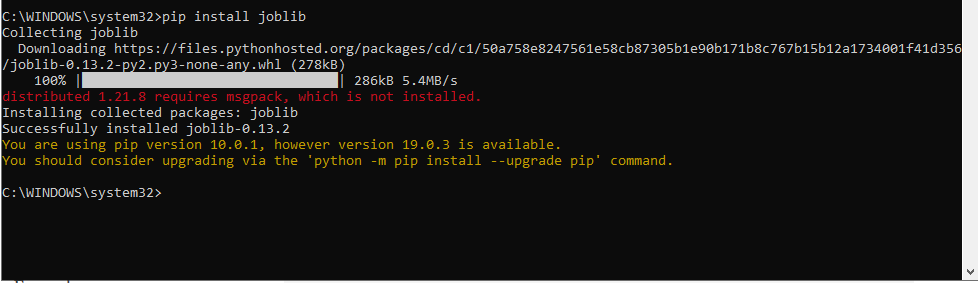
\includegraphics[scale=0.5]{figures/i21.png}
\caption{Error}
\end{figure}

\item Untuk itu solusinya saya install terlebih dahulu joblib agar error pun tidak terjadi kembali.
\end{itemize}

\begin{figure}[ht]
\centering
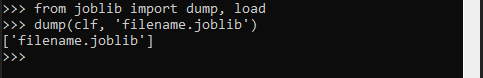
\includegraphics[scale=0.5]{figures/i22.png}
\caption{Error}
\end{figure}

